\documentclass[12pt]{exam}
\usepackage{amsthm}
\usepackage{bm}
\usepackage{libertine}
\usepackage[utf8]{inputenc}
\usepackage[margin=0.5in]{geometry}
\usepackage{amsmath,amssymb}
\usepackage{multicol}
\usepackage[shortlabels]{enumitem}
\usepackage{siunitx}
\usepackage{physics}
\usepackage{booktabs}
\usepackage{graphicx}
\usepackage{pgfplots}
\usepackage{listings}
\usepackage{tikz}
\usepackage{tikz-3dplot}

\bmdefine{\ii}{i}
\bmdefine{\jj}{j}
\bmdefine{\kk}{k}
\newcommand{\te}{\theta}
\newcommand{\cC}{\mathcal{C}}
\newcommand{\word}[1]{\quad\text{#1}\quad}

\pgfplotsset{width=10cm,compat=1.9}
\usepgfplotslibrary{external}
\tikzexternalize
% The existing black-and-white standalone figure is included as a PDF.
\tikzexternaldisable

\newcommand{\class}{Math 261-001}
\newcommand{\examnum}{Quiz 6 Solutions}
% Assumed quiz date: the next weekly Friday after October 8, 2026.
\newcommand{\examdate}{October 9}

\begin{document}
\pagestyle{plain}
\thispagestyle{empty}

\noindent
\textbf{\class}\\
\textbf{\examnum}, \textbf{\examdate}

\vspace{8pt}
\small
\setlength{\abovedisplayskip}{6pt}
\setlength{\belowdisplayskip}{6pt}
\setlength{\abovedisplayshortskip}{3pt}
\setlength{\belowdisplayshortskip}{6pt}
\begin{enumerate}

\item \textbf{Final answer:} $\boxed{\pi(2-\sqrt2)\ln2}$.

Use spherical coordinates
\[
  x=\rho\sin\varphi\cos\theta,\qquad
  y=\rho\sin\varphi\sin\theta,\qquad
  z=\rho\cos\varphi,
\]
where $\varphi$ is measured from the positive $z$-axis.
The sphere inequalities give $1\leq\rho\leq2$.
Since $\rho>0$, the cone inequality becomes
$\rho\cos\varphi\geq\rho\sin\varphi$, so
$0\leq\varphi\leq\pi/4$. There is no azimuthal restriction.
The Cartesian conditions and the spherical bounds are
\[
  \left\{
  \begin{aligned}
    &1\leq x^2+y^2+z^2\leq4,\\
    &z\geq\sqrt{x^2+y^2}
  \end{aligned}
  \right.
  \qquad\Longrightarrow\qquad
  \left\{
  \begin{aligned}
    &0\leq\theta\leq2\pi,\\
    &0\leq\varphi\leq\pi/4,\\
    &1\leq\rho\leq2.
  \end{aligned}
  \right.
\]
The integrand is $\rho^{-3}$, and the volume element is
$dV=\rho^2\sin\varphi\,d\rho\,d\varphi\,d\theta$.
Consequently,
\[
\begin{aligned}
  I&=\int_0^{2\pi}\int_0^{\pi/4}\int_1^2
      \frac{\sin\varphi}{\rho}\,d\rho\,d\varphi\,d\theta\\
   &=2\pi\,[{-\cos\varphi}]_0^{\pi/4}\,[\ln\rho]_1^2
     =2\pi\left(1-\frac1{\sqrt2}\right)\ln2
     =\pi(2-\sqrt2)\ln2.
\end{aligned}
\]
The result is positive, as expected; the inner sphere excludes the
singularity at the origin.

\smallskip
\textit{Full credit:} any exact expression equal to $\pi(2-\sqrt2)\ln2$,
including $2\pi(1-1/\sqrt2)\ln2$. An unevaluated integral alone is
incomplete. Equivalent full-turn $\theta$-intervals give the same setup.

\medskip
\item \textbf{Final answer:} $\boxed{S=4\pi}$.

For the fly's path,
\[
\begin{aligned}
  \vec r(t)&=(\cos t,\sin t,2+\cos t+\sin t),\\
  \vec r\,'(t)&=(-\sin t,\cos t,\cos t-\sin t),\\
  \|\vec r\,'(t)\|
    &=\sqrt{\sin^2t+\cos^2t+(\cos t-\sin t)^2}
     =\sqrt{1+(\cos t-\sin t)^2}.
\end{aligned}
\]
The scent intensity along the path is
\[
  \sigma(\vec r(t))=\sqrt{1+(\cos t-\sin t)^2}
     =\|\vec r\,'(t)\|.
\]
For a scalar line integral, multiply the scalar field by the speed:
$ds=\|\vec r\,'(t)\|\,dt$, not just $dt$. Thus
\[
\begin{aligned}
  S&=\int_0^{2\pi}\sigma(\vec r(t))\|\vec r\,'(t)\|\,dt\\
   &=\int_0^{2\pi}\bigl(1+(\cos t-\sin t)^2\bigr)\,dt
     =\int_0^{2\pi}(2-\sin2t)\,dt\\
   &=\left[2t+\tfrac12\cos2t\right]_0^{2\pi}=4\pi.
\end{aligned}
\]
This is scent intensity weighted by distance traveled, not a time integral
of scent intensity. Reversing the flight direction would not change this
scalar line integral.

\smallskip
\textit{Full credit:} any exact expression equal to $4\pi$.
An unevaluated integral alone is incomplete.

\newpage

\item \textbf{Final answer:} $\boxed{-2}$.

The path follows increasing $t$ from $(\pi/2,\pi^2/4)$ to $(\pi,\pi^2)$.
Substitute $x=t$, $y=t^2$ into both components of the field:
\[
  \vec F(\vec r(t))
    =\left(\frac{t^2\cos t}{t^2},-\frac{\sin t}{2t}\right)
    =\left(\cos t,-\frac{\sin t}{2t}\right),
  \qquad \vec r\,'(t)=(1,2t).
\]
Here $t\geq\pi/2>0$, so the denominators never vanish. The vector
line integral uses the dot product with $\vec r\,'(t)$:
\[
\begin{aligned}
  \int_C\vec F\cdot d\vec r
    &=\int_{\pi/2}^{\pi}\vec F(\vec r(t))\cdot\vec r\,'(t)\,dt\\
    &=\int_{\pi/2}^{\pi}(\cos t-\sin t)\,dt
      =[\sin t+\cos t]_{\pi/2}^{\pi}=-1-1=-2.
\end{aligned}
\]
Do not insert an additional speed factor: $d\vec r=\vec r\,'(t)\,dt$.
Reversing the orientation would give $+2$, which is not the requested
integral.

\smallskip
\textit{Full credit:} any exact expression equal to $-2$.
An unevaluated integral alone is incomplete.

\medskip
\item \textbf{Final answers:}
\begin{center}
\begin{tabular}{@{}ccc@{}}
\toprule
Square & Field relative to the oriented tangent & Contribution\\
\midrule
A & Opposite direction & Negative ($-$)\\
B & Perpendicular & Zero ($0$)\\
C & Same direction & Positive ($+$)\\
\bottomrule
\end{tabular}
\end{center}
For the oriented unit tangent $\vec T$, the infinitesimal contribution is
$\vec F\cdot\vec T\,ds$. The path's filled arrowheads determine $\vec T$;
the thinner dashed arrows represent $\vec F$. Opposite, perpendicular,
and matching directions give negative, zero, and positive dot products,
respectively. These alignments hold throughout each highlighted piece,
so the signs also describe the integrals over those pieces.

\medskip
\noindent\begin{minipage}[c]{0.50\linewidth}
\centering
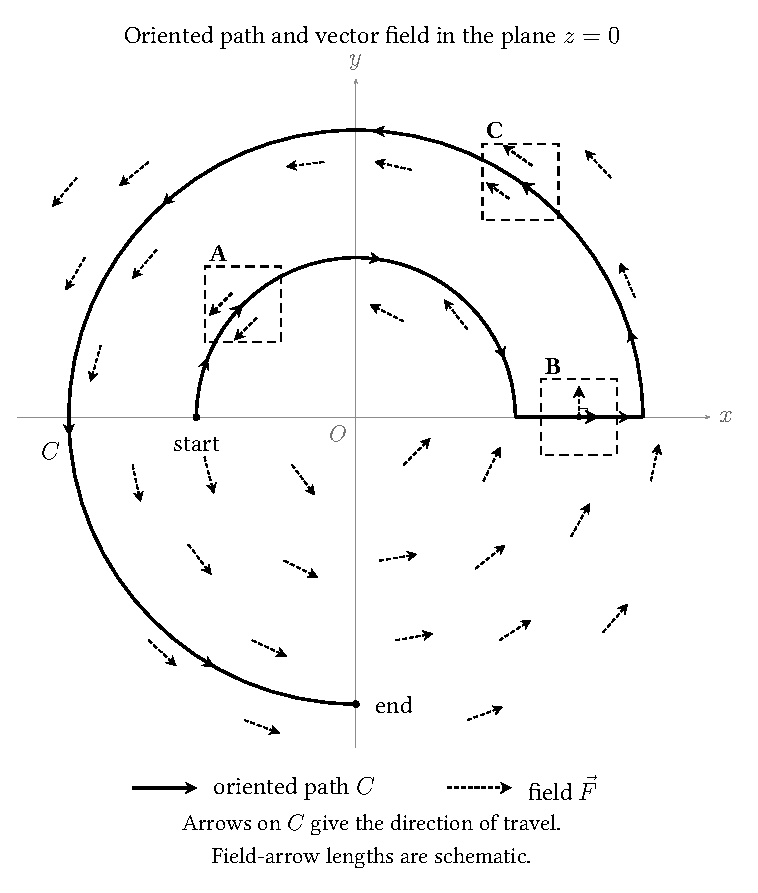
\includegraphics[width=9cm]{figures/q6-field-signs.pdf}
\end{minipage}\hfill
\begin{minipage}[c]{0.46\linewidth}
\raggedright
\textit{Instructor check:} the hidden field is $\vec F(x,y,z)=(-y,x,0)$.
Its dot product with the oriented unit tangent is $-2$ on the inner
clockwise arc, $0$ on the outward radial segment, and $18/5$ on the
outer counterclockwise arc. Arrow lengths in the drawing are schematic.

\medskip
\textit{Full credit:} A negative, B zero, C positive, accepting either
words or the symbols $-,0,+$ in the corresponding entries. Treat the
three entries as equally weighted components; no written explanation is
required. The question does not ask for the sign over the entire path.
\end{minipage}

\end{enumerate}
\end{document}
